% 2018 江苏卷第21题【A】：圆切线与割线
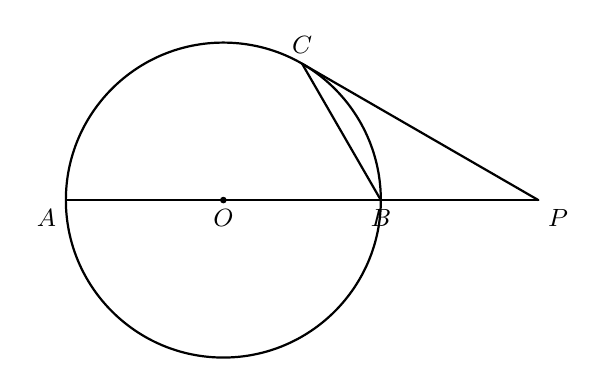
\begin{tikzpicture}[font=\small, line cap=round, line join=round, >=stealth, scale=1.0]
  % 圆心与半径 R = 2
  \coordinate (O) at (0, 0);
  \draw[thick] (O) circle (2cm);

  % 直径 AB: A(-2, 0), B(2, 0)
  \coordinate (A) at (-2, 0);
  \coordinate (B) at (2, 0);

  % P 在 AB 延长线上，P(4, 0)
  \coordinate (P) at (4, 0);
  \draw[thick] (A) -- (P);

  % 切点 C: (1, sqrt(3))
  \coordinate (C) at (1, 1.732);

  % 切线 PC 与 弦 BC
  \draw[thick] (P) -- (C);
  \draw[thick] (B) -- (C);

  % 标签与点
  \fill (O) circle (1.2pt) node[below] {$O$};
  \node[below left] at (A) {$A$};
  \node[below] at (B) {$B$};
  \node[below right] at (P) {$P$};
  \node[above] at (C) {$C$};
\end{tikzpicture}
